\chapter{Materials and Methods}

\section{Datasets}

The dataset utilized in this study was provided by the supervisor and obtained by the company Ornavera. Ornavera is dedicated to generating actionable data insights for agricultural health. Their mission is to create tools for data collection in agriculture, automating mathematical and scientific processes to benefit farmers through artificial intelligence and precision agriculture.

\subsection{ORNAVERA Data Collection Device (DCD)}

The DCD is responsible for gathering and transmitting data from various geo-physical and plant sensors to the Ornavera Data Aggregation Device (DAD) using a certified LoRa® radio interface.
\begin{figure}[htbp]
    \centering
    \includegraphics[width=6 cm]{4_ChapterMaterials/figuras/DCDornavera.pdf}
    \caption{ORNAVERA Data Collection Device (DCD)\cite{ornavera2020dcd}}
    \LABFIG{FIG}
    \end{figure}

It features:
\begin{itemize}
    \item \textbf{Wireless Interface:} Utilizes LoRa® technology for long-range, low-power communication with a coverage radius of up to 15 km in rural areas and 5 km in urban areas.
    \item \textbf{Controller:} Equipped with a high-performance ARM® Cortex® microcontroller for efficient data handling and communication.
    \item \textbf{Power Supply:} Operates on a solar-assisted Li-ion battery with a backup life of 1-2 months depending on sensor usage.
    \item \textbf{Interfaces:} Supports multiple I2C, SPI, and RS485 connections for various sensors, with additional ports for future expansion.
    \item \textbf{Environmental Tolerance:} Designed to operate within a temperature range of -10°C to 55°C and humidity levels of 10\%-95\% RH.
\end{itemize}


The ORNAVERA Data Collection Device (DCD) is equipped with the following sensors:
\begin{itemize}
    \item \textbf{Temperature and Humidity Probe:} SHT20 from Sensirion, providing accurate measurements of ambient conditions around the pepper plant.
    \begin{figure}[htbp]
        \centering
        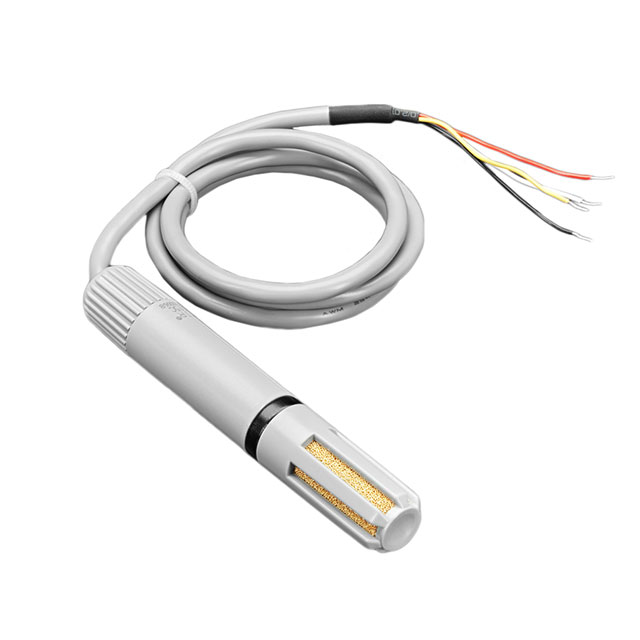
\includegraphics[width=6 cm]{4_ChapterMaterials/figuras/SHT20.jpg}
        \caption{Temperature and Humidity Probe: SHT20 from Sensirion\cite{ornavera2020dcd}}
        \LABFIG{FIG}
        \end{figure}

    \item \textbf{Soil Probe:} MEC-10, measuring soil moisture, pH, and other critical parameters for assessing soil health and suitability for pepper cultivation.
    \begin{figure}[htbp]
        \centering
        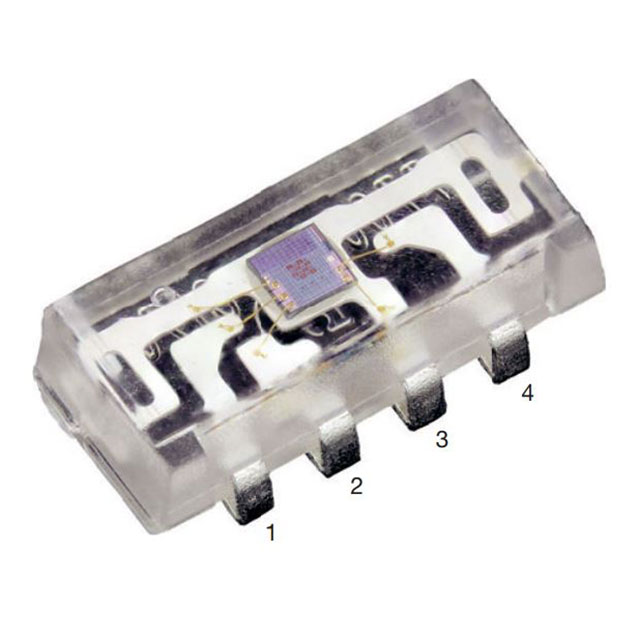
\includegraphics[width=6 cm]{4_ChapterMaterials/figuras/VEML7700.jpeg}
        \caption{Soil Probe: MEC-10 from Dalian Endeavour Technology Co. \cite{ornavera2020dcd}}
        \LABFIG{FIG}
        \end{figure}

    \item \textbf{Light Sensor:} VEML7700 from Vishay, used to measure light intensity impacting the pepper plant.
    \begin{figure}[htbp]
        \centering
        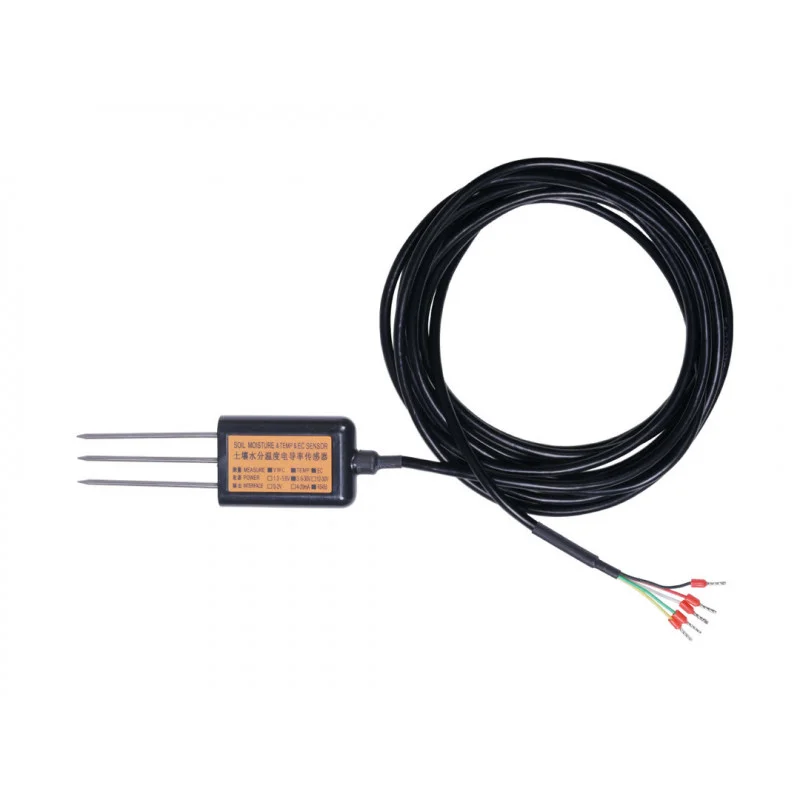
\includegraphics[width=6 cm]{4_ChapterMaterials/figuras/MEC10.png}
        \caption{Light Sensor: VEML7700 from Vishay.\cite{ornavera2020dcd}}
        \LABFIG{FIG}
        \end{figure}

    \item \textbf{Dendrometer:} Designed by Ornavera, used to measure the diameter of the pepper plant, essential for tracking its growth.
\end{itemize}


These sensors, integrated with the DCD, provided a detailed dataset for analyzing the environmental and soil conditions affecting pepper plant growth. The data collected was carefully recorded and analyzed to draw valuable insights for the study.


\section{Available Variables}

Thanks to the sensors mentioned previously, we have been able to extract a set of crucial variables for analyzing the growth of pepper plants. These data allow us to accurately assess the environmental and soil conditions that influence plant development. In the following section, the importance of these variables in plant growth is explained, highlighting how each one contributes to a better understanding of the agricultural environment and the optimization of cultivation practices.

\subsection{Temperature (t1)}

Temperature is a fundamental factor influencing plant growth, as it affects critical physiological processes such as photosynthesis, respiration, and transpiration. The variable \( t1 \) measures the ambient air temperature surrounding the plant, which is essential for determining whether environmental conditions are conducive to optimal growth. For instance, most plants have a specific temperature range within which they perform best. Outside this range, physiological processes can become less efficient, potentially leading to stress. For example, excessively high temperatures can increase respiration rates to the detriment of photosynthesis, ultimately hindering plant growth. Conversely, low temperatures can slow down metabolic activities, leading to reduced growth rates. Therefore, maintaining optimal temperature conditions can enhance the overall productivity and health of plants, making it a crucial variable to monitor.

\begin{figure}[htbp]
    \centering
    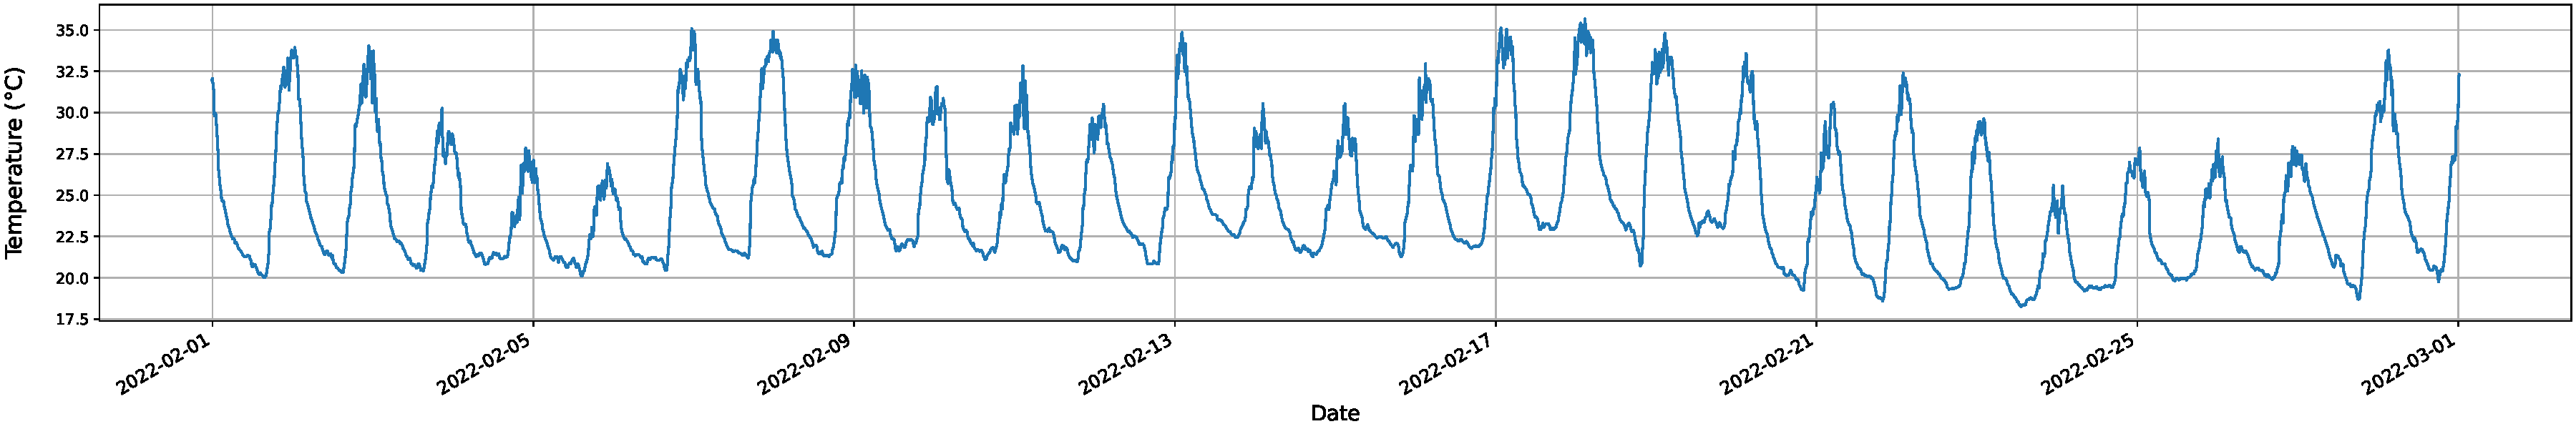
\includegraphics[width=15 cm]{4_ChapterMaterials/figuras/train_data_Temperature.pdf}
    \caption{Graph of Temperature Measurements for February}
    \LABFIG{FIG}
    \end{figure}

\subsection{Relative Humidity (rh1)}

Relative humidity (\( rh1 \)) is another critical environmental factor, representing the percentage of moisture in the air relative to the maximum amount the air can hold at a given temperature. It plays a significant role in plant water use efficiency and disease management. High relative humidity can reduce transpiration rates, which might lead to an accumulation of water in the plant and potentially create conditions for disease, particularly fungal infections. Conversely, low humidity levels can cause increased transpiration, leading to water stress if not balanced by sufficient water uptake from the soil. Properly managing humidity levels is crucial for optimizing plant health, as it impacts everything from water uptake to disease resistance. Understanding relative humidity patterns allows farmers to adjust irrigation practices and greenhouse conditions to improve crop resilience and productivity.

\begin{figure}[htbp]
    \centering
    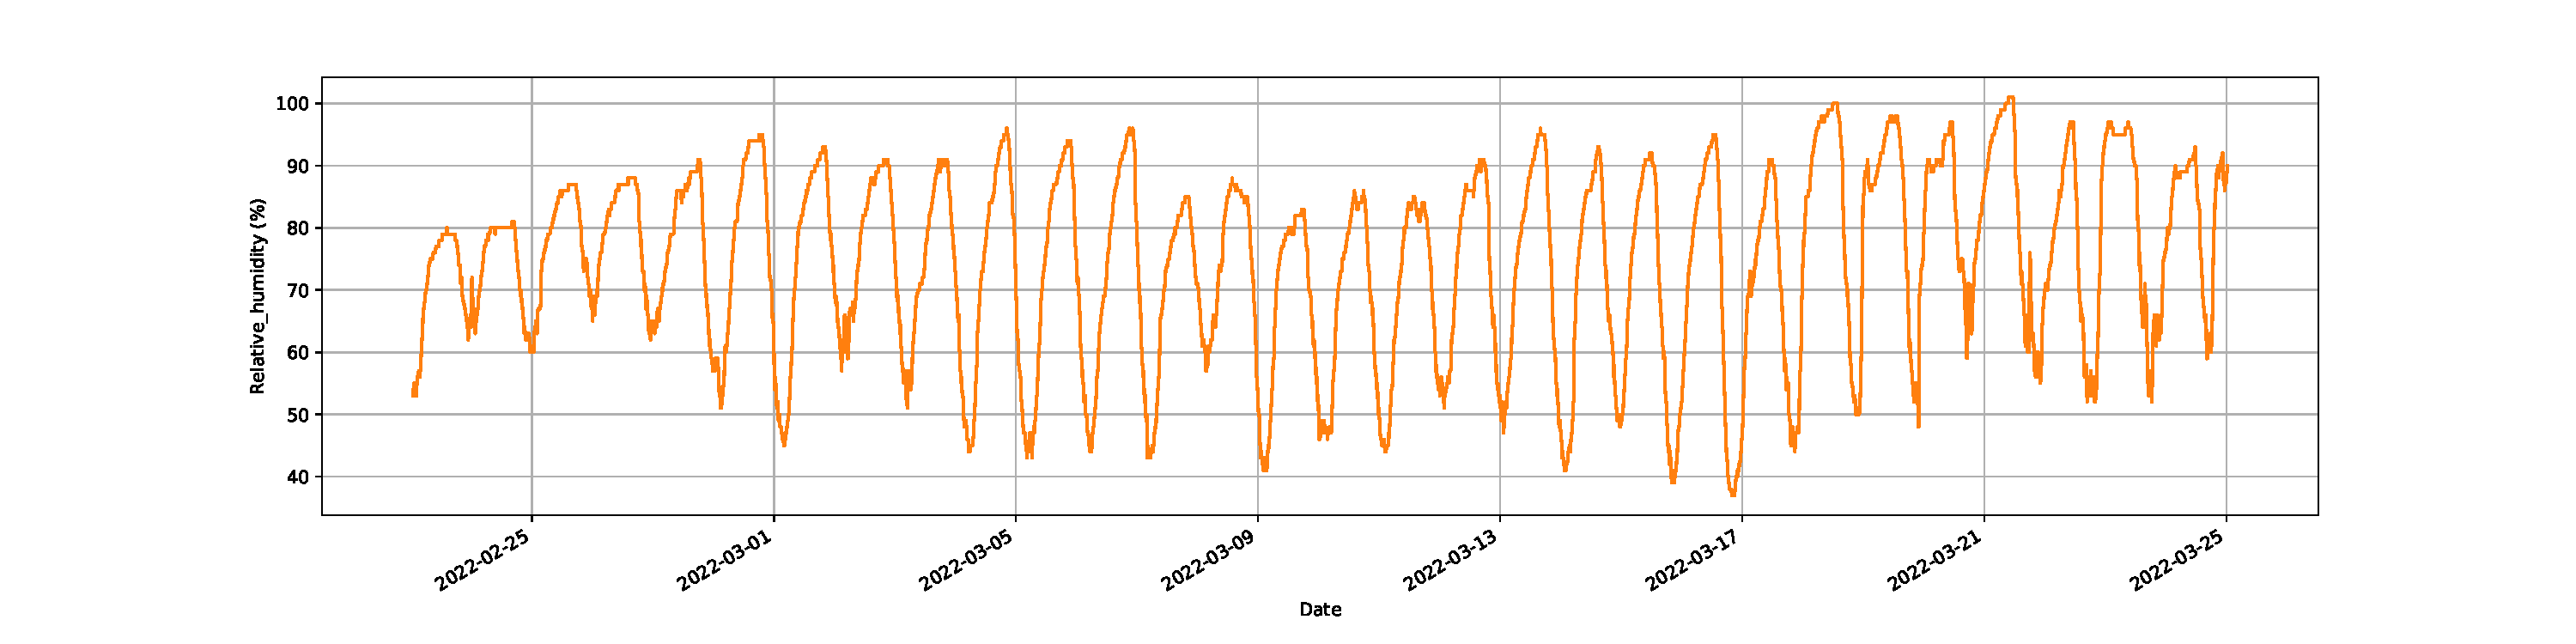
\includegraphics[width=15 cm]{4_ChapterMaterials/figuras/train_data_Relative_humidity.pdf}
    \caption{Graph of Relative Humidity Measurements for February}
    \LABFIG{FIG}
    \end{figure}

\subsection{Vapor Pressure Deficit (vpd1)}

Vapor Pressure Deficit (VPD), derived from relative humidity and temperature, provides insights into the drying power of the air. It represents the difference between the amount of moisture in the air and how much moisture the air can hold when saturated. This measure is crucial for understanding plant transpiration rates and water stress levels. High VPD indicates drier air, which can increase transpiration and potentially lead to water stress if not adequately managed. On the other hand, low VPD suggests more humid conditions, which can reduce transpiration and, in some cases, lead to an excess of moisture around the plant, fostering mold and mildew. By monitoring VPD, growers can make informed decisions about irrigation and climate control, ensuring plants receive the optimal balance of moisture to thrive.

\begin{figure}[htbp]
    \centering
    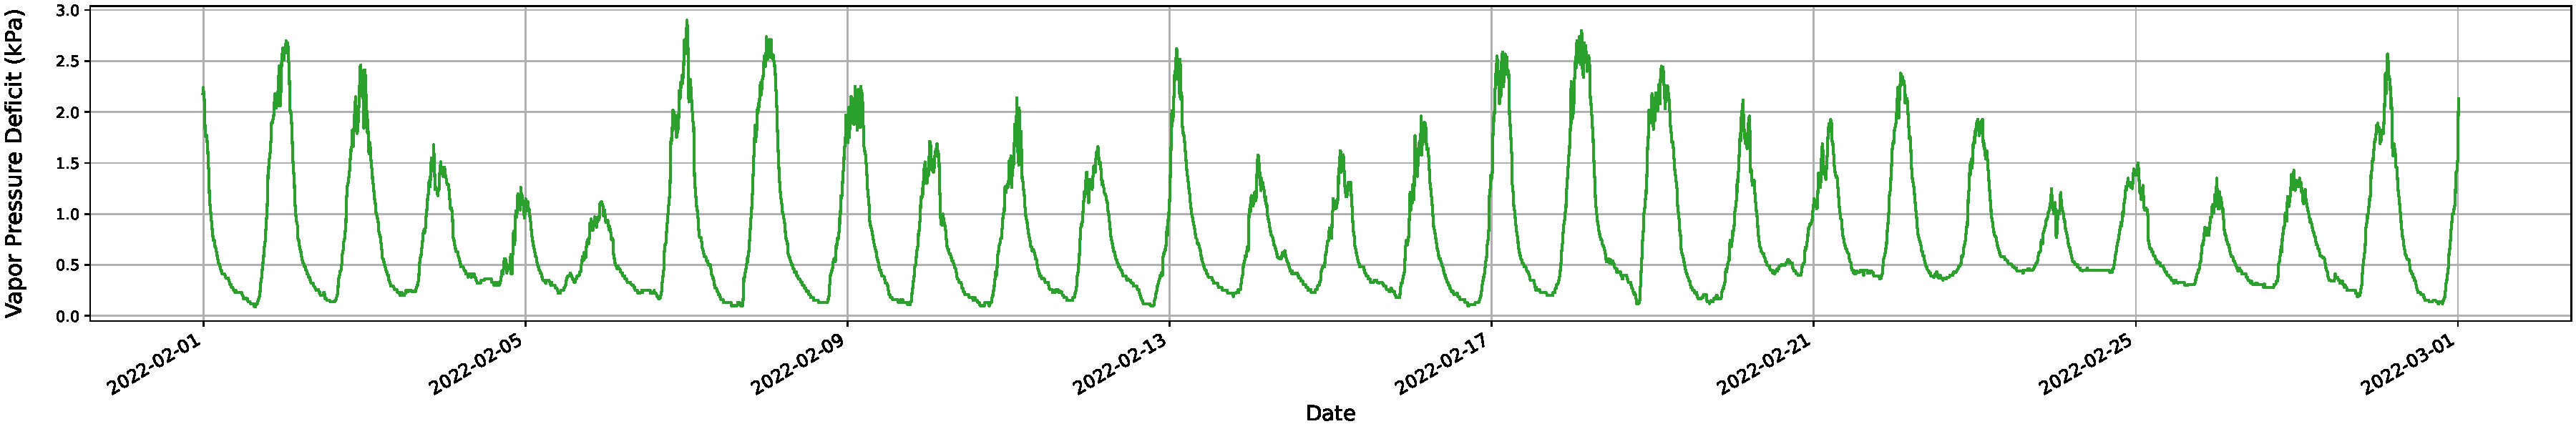
\includegraphics[width=15 cm]{4_ChapterMaterials/figuras/train_data_Vapor_Pressure_Deficit.pdf}
    \caption{Graph of Vapor Pressure Deficit Measurements for February}
    \LABFIG{FIG}
    \end{figure}

\subsection{Light Intensity (lux)}

Light intensity, measured in lumens (lux), is crucial for plant growth as it directly impacts photosynthesis—the process by which plants convert light into energy. Adequate light intensity is essential for driving this process, influencing growth rates and overall plant health. Insufficient light can limit photosynthesis, stunting growth and leading to weaker plants, while excessive light can cause photoinhibition, where too much light actually damages the photosynthetic apparatus, reducing efficiency. Understanding and managing light exposure is therefore vital for maximizing photosynthetic activity, especially in controlled environments like greenhouses. By ensuring that plants receive the right amount of light, farmers can enhance growth rates, improve flowering and fruiting patterns, and optimize crop yields.

\begin{figure}[htbp]
    \centering
    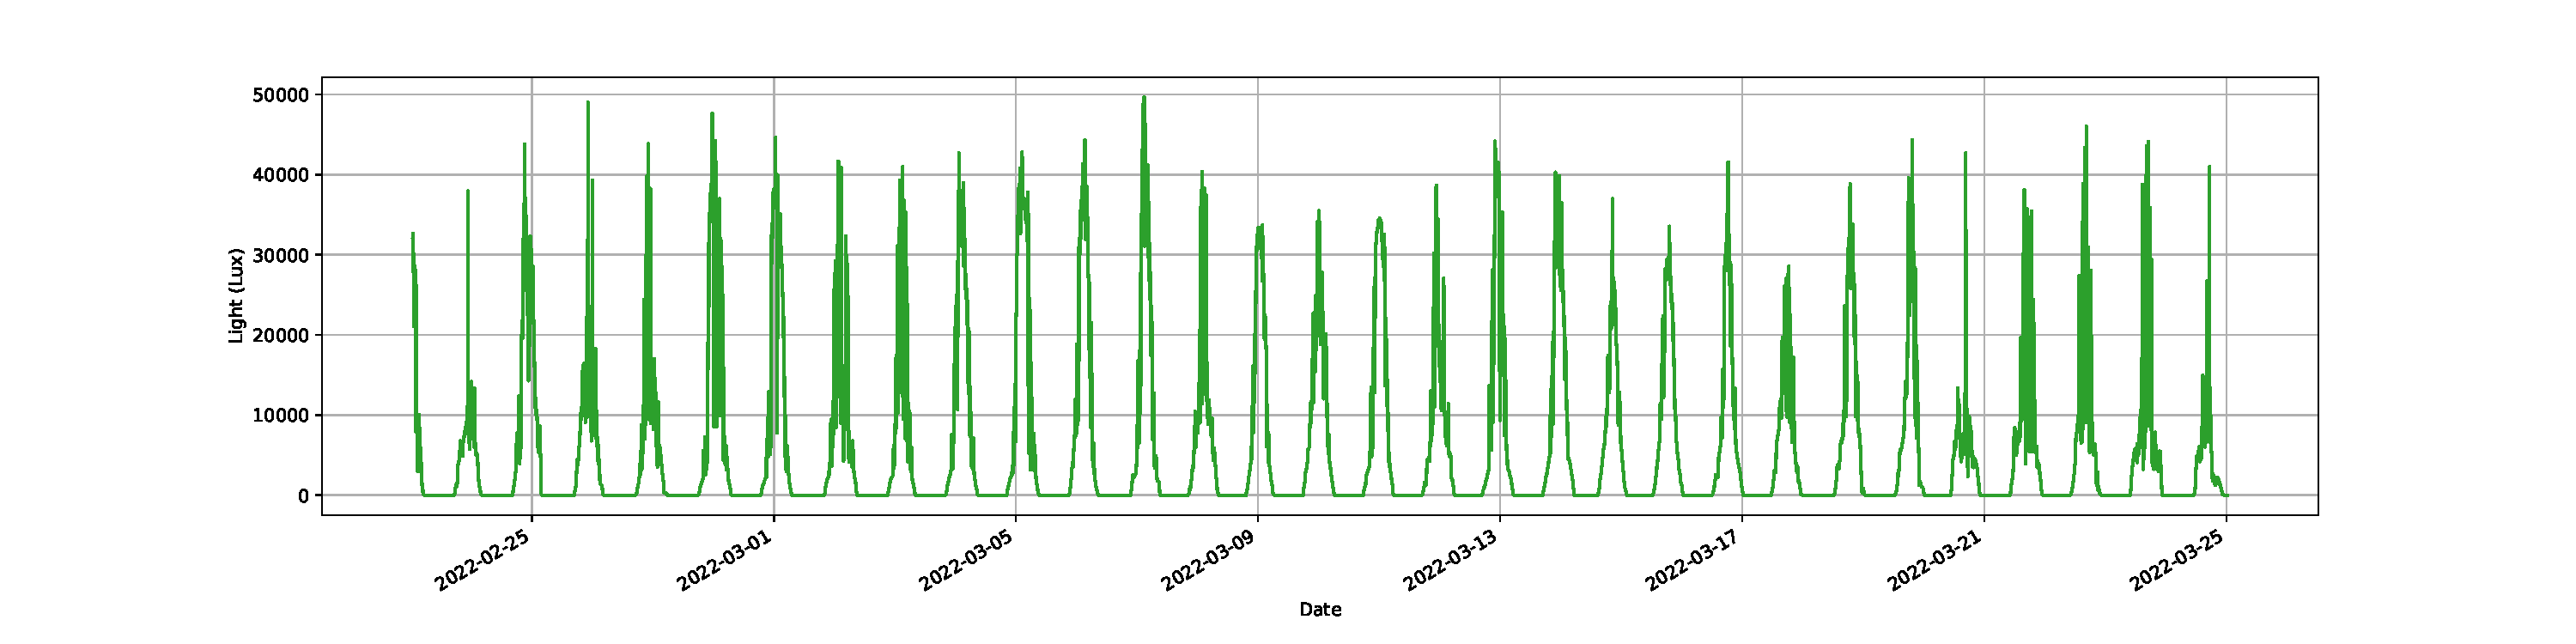
\includegraphics[width=15 cm]{4_ChapterMaterials/figuras/train_data_Light.pdf}
    \caption{Graph of Light Intensity Measurements for February}
    \LABFIG{FIG}
    \end{figure}

\subsection{Soil Temperature (st1)}

Soil temperature (\( st1 \)) is a key variable that influences root activity and microbial processes in the soil, both of which are critical for nutrient uptake and plant growth. Soil temperature affects root metabolism, with optimal temperatures promoting vigorous root growth and nutrient absorption. If soil temperatures fall outside the optimal range, root activity can slow down, impairing the plant's ability to access water and nutrients, and potentially leading to stunted growth. Additionally, soil temperature affects the activity of soil microbes, which play a vital role in decomposing organic matter and releasing nutrients in forms that plants can absorb. Monitoring soil temperature helps in managing planting schedules and optimizing root zone conditions to ensure that plants have access to the nutrients they need for healthy growth and development.

\begin{figure}[htbp]
    \centering
    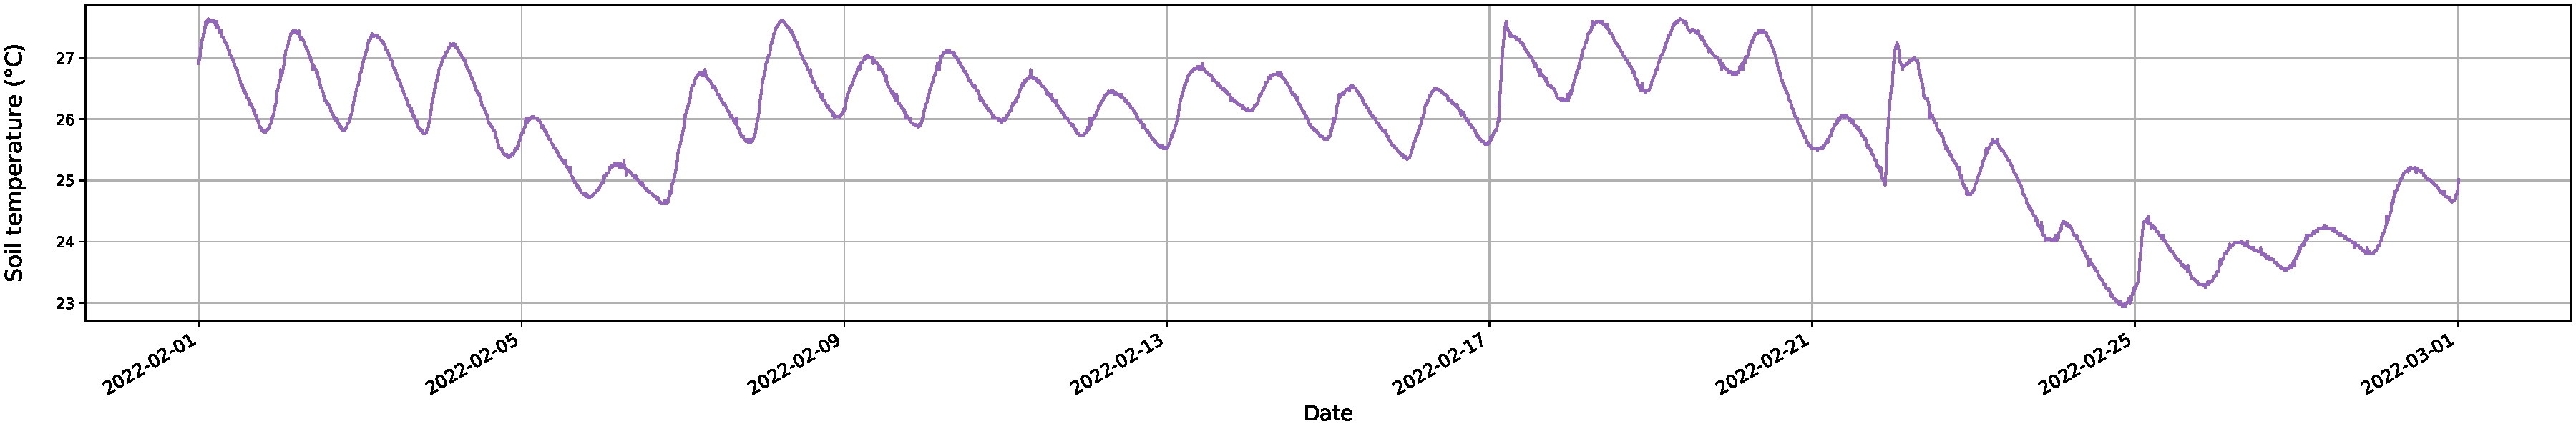
\includegraphics[width=15 cm]{4_ChapterMaterials/figuras/train_data_Soil_temperature.pdf}
    \caption{Graph of Soil Temperature Measurements for February}
    \LABFIG{FIG}
    \end{figure}

\subsection{Permittivity (p1)}

Permittivity is a measure of a soil's ability to store and transmit electric fields, closely related to its moisture content. High permittivity often indicates a higher soil moisture level, which is crucial for nutrient transport and root uptake. Adequate soil moisture facilitates the movement of nutrients from the soil to the plant roots, thereby supporting healthy growth. However, too much moisture can lead to waterlogged conditions, which can suffocate roots and inhibit their ability to function properly. By measuring permittivity, growers can gain insights into soil moisture levels and make informed decisions about irrigation practices. This ensures that plants receive the optimal amount of water, reducing stress and enhancing growth conditions, which is particularly important for maintaining crop health in varying weather conditions.

\begin{figure}[htbp]
    \centering
    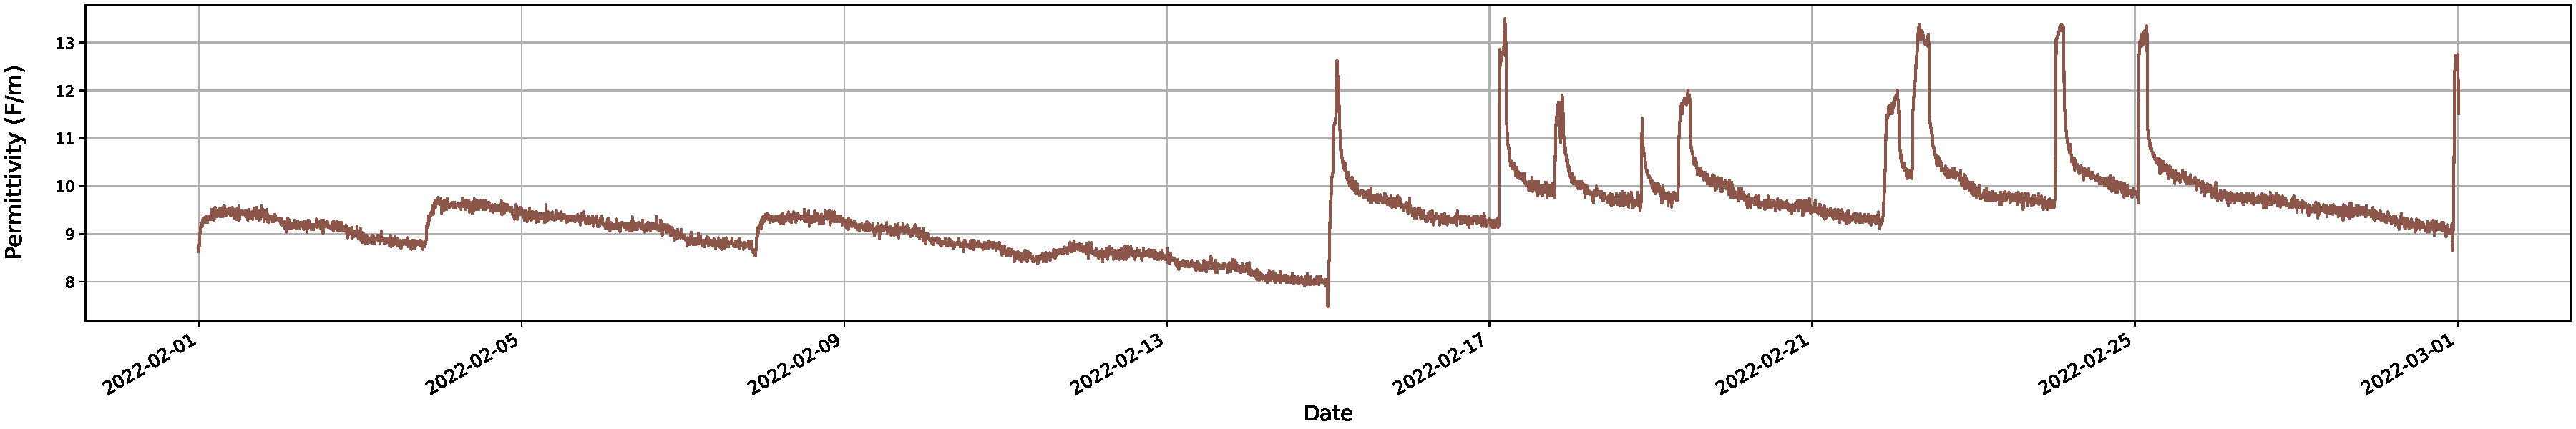
\includegraphics[width=15 cm]{4_ChapterMaterials/figuras/train_data_Permittivity.pdf}
    \caption{Graph of Permittivity Measurements for February}
    \LABFIG{FIG}
    \end{figure}

\subsection{Electrical Conductivity (ec1)}

Electrical conductivity (\( ec1 \)) measures the soil's ability to conduct electricity, which is indicative of the concentration of soluble salts and nutrients in the soil. High electrical conductivity can indicate excessive salts, which may lead to osmotic stress and interfere with nutrient uptake. This can harm plant growth, especially in crops sensitive to salinity. On the other hand, low electrical conductivity may suggest nutrient deficiencies that can limit growth and yield. Monitoring electrical conductivity is essential for diagnosing soil fertility and salinity issues, allowing farmers to adjust fertilization practices accordingly. By maintaining balanced nutrient levels, plants can achieve optimal growth and productivity, highlighting the importance of regular soil EC monitoring.

\begin{figure}[htbp]
    \centering
    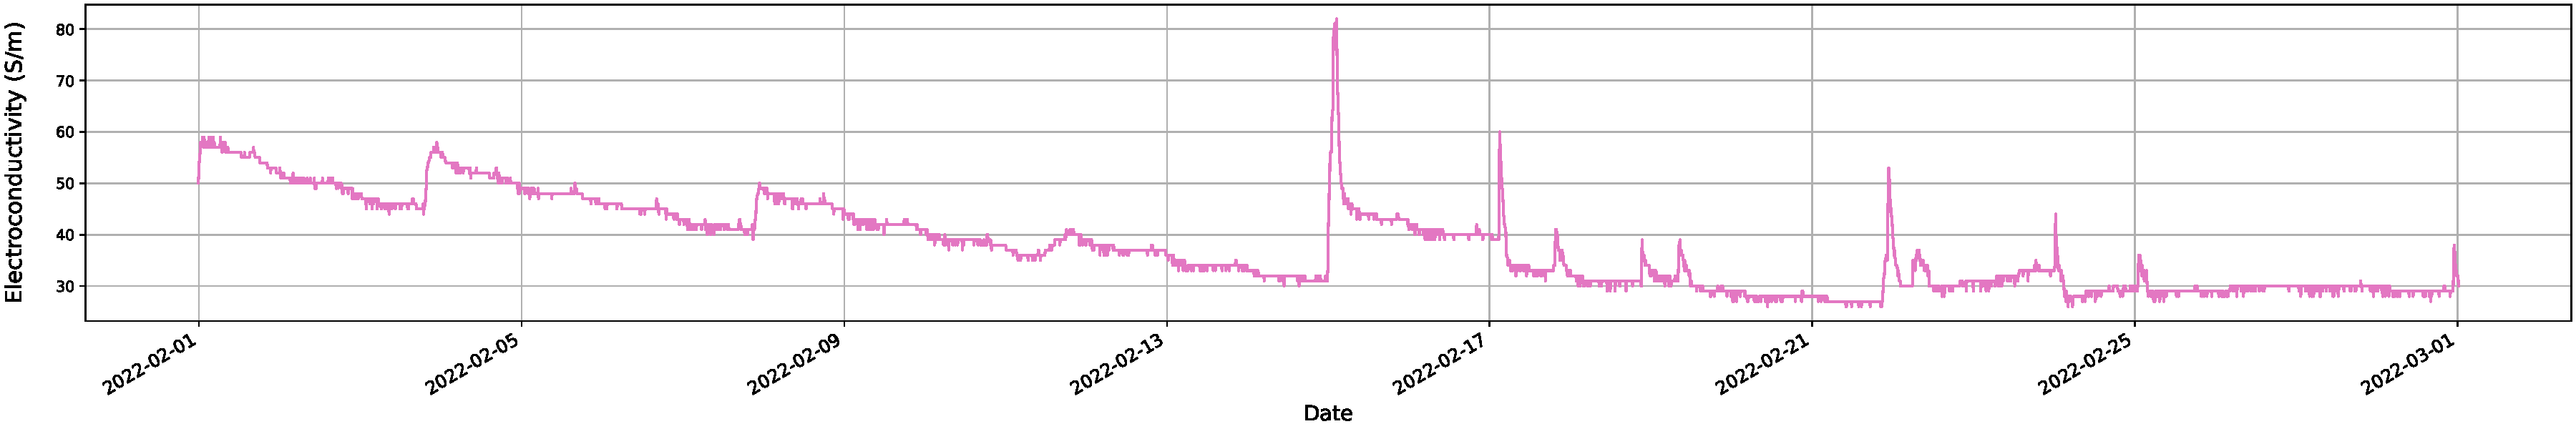
\includegraphics[width=15 cm]{4_ChapterMaterials/figuras/train_data_Electroconductivity.pdf}
    \caption{Graph of Electroconductivity Measurements for February}
    \LABFIG{FIG}
    \end{figure}

\subsection{Volumetric Water Content (vwc1)}

Volumetric Water Content (\( vwc1 \)) measures the percentage of water present in the soil, reflecting the soil moisture status and availability for plant uptake. This variable is crucial for understanding the water dynamics within the soil and ensuring plants have sufficient water for physiological processes. Adequate soil moisture supports nutrient uptake and maintains plant turgor, which is vital for growth and stability. However, both insufficient and excessive moisture can cause stress: too little water can lead to drought stress, while too much can lead to root rot and decreased oxygen availability. By monitoring volumetric water content, growers can fine-tune irrigation practices to maintain optimal soil moisture levels, improving plant health, conserving water, and ensuring efficient use of resources.

\begin{figure}[htbp]
    \centering
    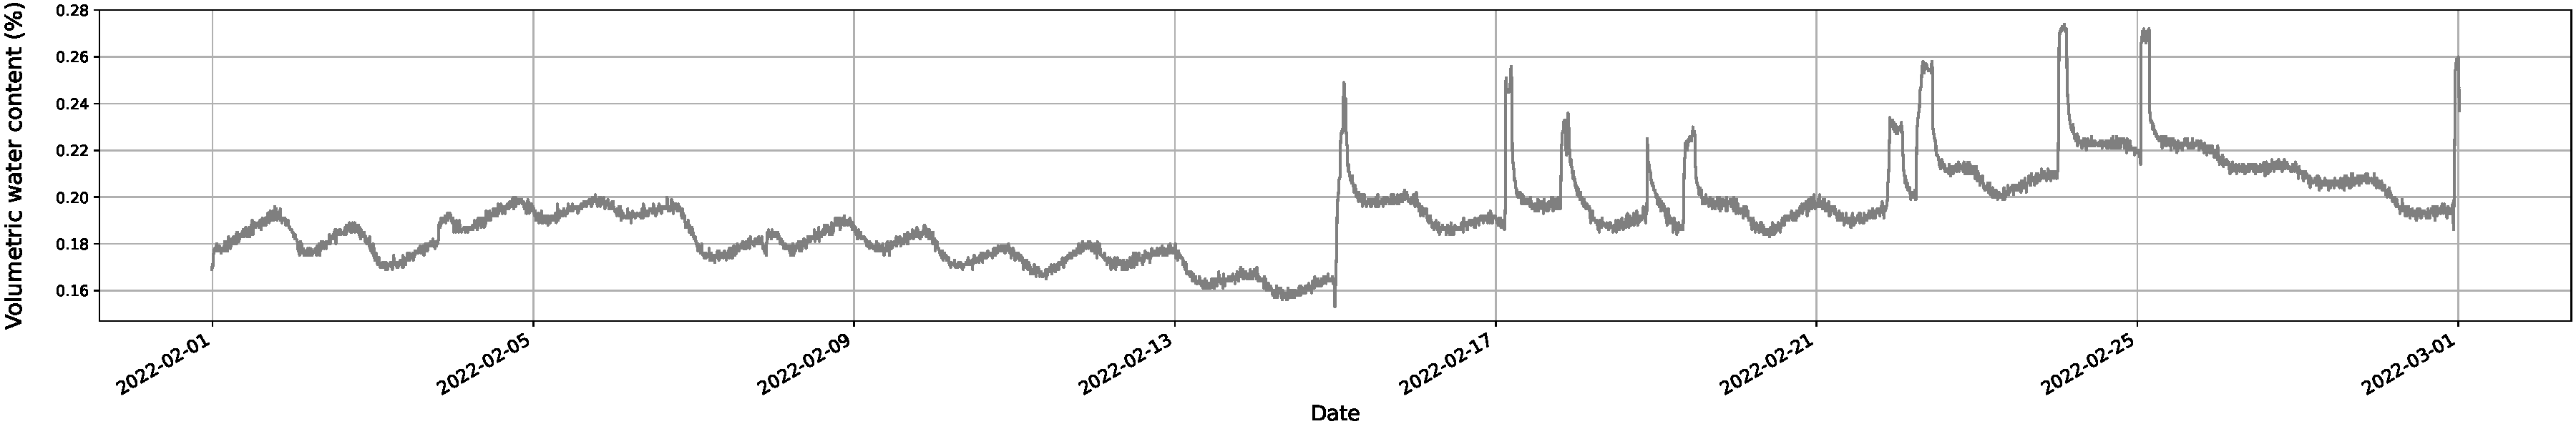
\includegraphics[width=15 cm]{4_ChapterMaterials/figuras/train_data_Volumetric_water_content.pdf}
    \caption{Graph of Volumetric Water Content Measurements for February}
    \LABFIG{FIG}
    \end{figure}

\subsection{Diameter (diam1)}

The diameter of a plant's stem (\( diam1 \)) serves as a practical measure of its growth vigor and overall health. An increasing diameter generally indicates healthy growth and biomass accumulation, reflecting the plant's ability to assimilate nutrients and convert them into structural tissues. Consistent monitoring of stem diameter can reveal growth trends and potentially highlight stress conditions before they become severe. For instance, a sudden decrease in growth rate might indicate a nutrient deficiency, water stress, or pest problem. Additionally, a thicker stem provides better structural support for the plant, enabling it to withstand environmental stresses and support fruit load. By measuring changes in diameter, farmers can assess plant health and make timely interventions to support optimal growth conditions.

\begin{figure}[htbp]
    \centering
    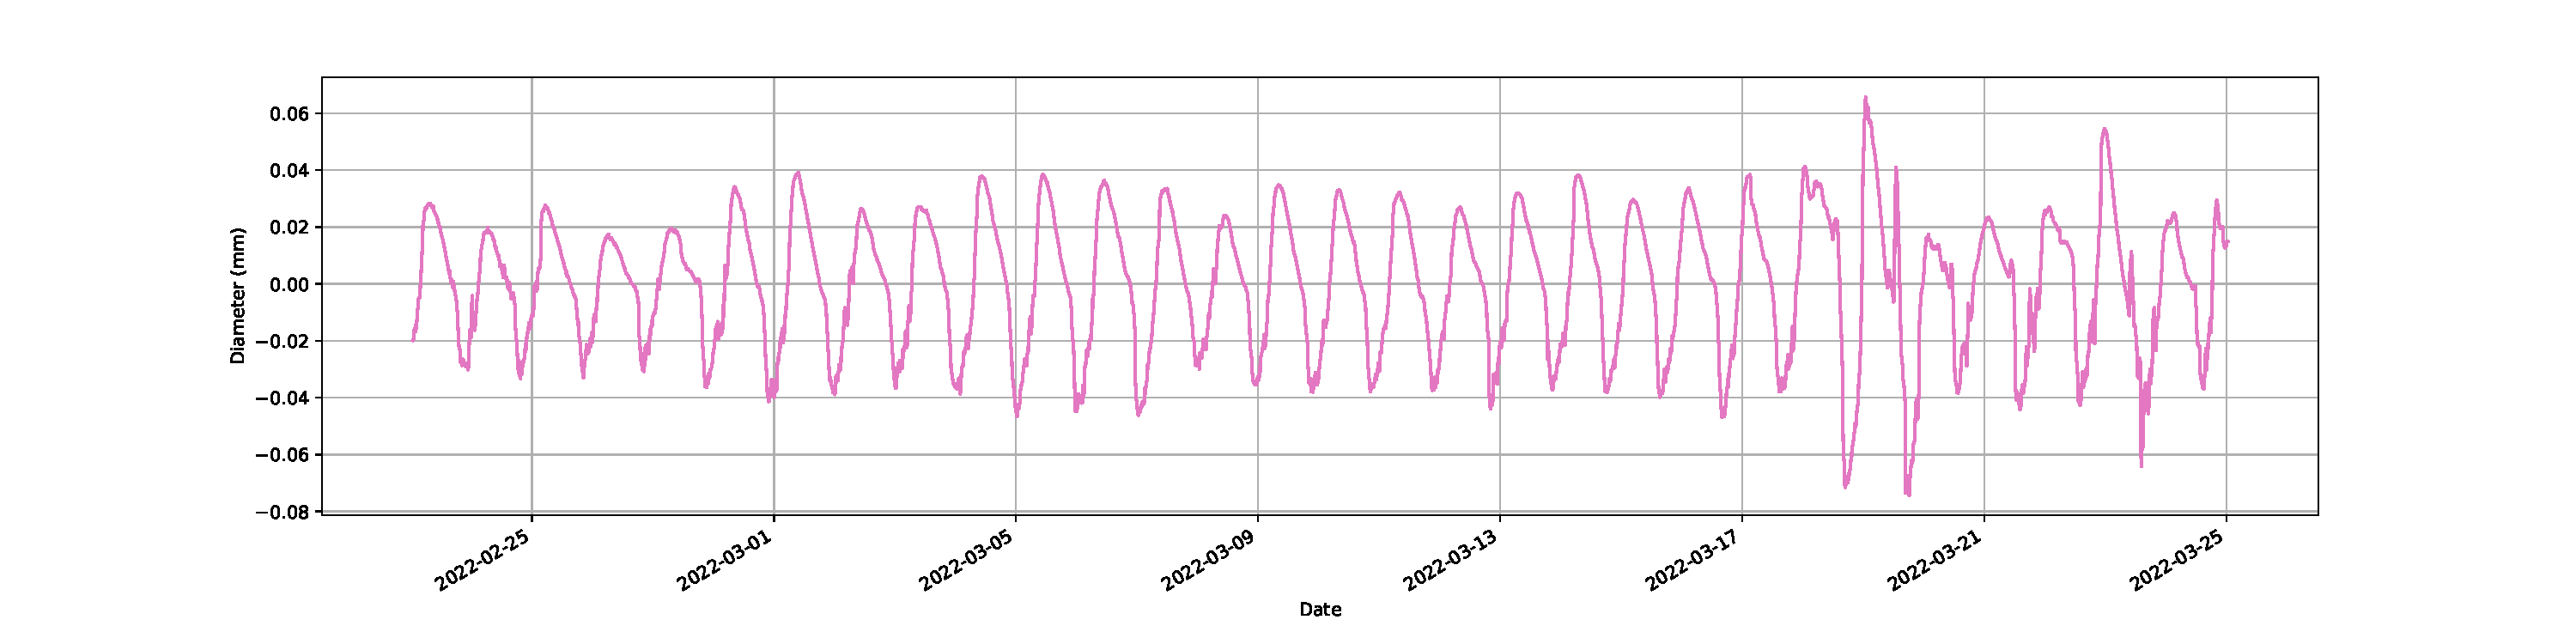
\includegraphics[width=15 cm]{4_ChapterMaterials/figuras/train_data_Diameter.pdf}
    \caption{Graph of Diameter Measurements for February}
    \LABFIG{FIG}
    \end{figure}

\subsection{Photosynthetically Active Radiation (par)}

Photosynthetically Active Radiation (PAR) is the portion of the light spectrum (400-700 nm) that plants use for photosynthesis. Unlike total light intensity, PAR specifically measures the wavelengths that drive photosynthesis, making it a more precise indicator of the light energy available for plant growth. The amount of PAR a plant receives directly influences its photosynthetic efficiency and, consequently, its growth and productivity. Variations in PAR can affect plant morphology, influencing factors such as leaf size, stem elongation, and flowering. By monitoring PAR, growers can optimize light conditions to ensure maximum photosynthetic activity, particularly in controlled environments like greenhouses where artificial lighting may be used. This helps in enhancing growth rates and improving yield quality, underscoring the importance of precise light management.

\begin{figure}[htbp]
    \centering
    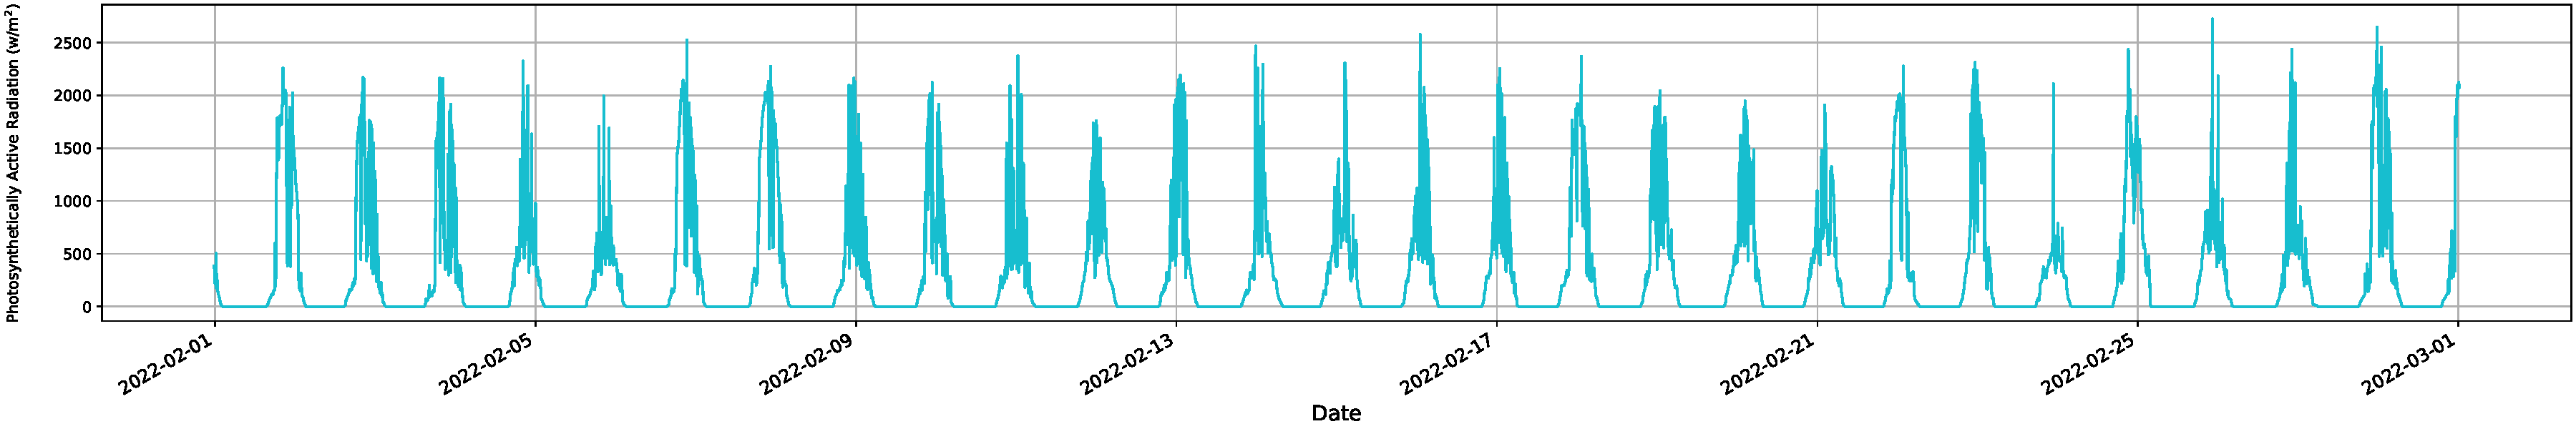
\includegraphics[width=15 cm]{4_ChapterMaterials/figuras/train_data_Photosynthetically_Active_Radiation.pdf}
    \caption{Graph of Photosynthetically Active Radiation Measurements for February}
    \LABFIG{FIG}
    \end{figure}

\section{Variable selection}

In the context of building an effective time series forecasting model for predicting changes in plant stem diameter, selecting the right variables is crucial for ensuring the model's accuracy and reliability. The process of variable selection is informed by both the theoretical understanding of plant physiology and empirical data analysis, specifically the correlation study conducted by Paula Fernández Yepes. In her research, a correlation matrix was calculated to evaluate the relationships between various environmental factors and the diameter of plants.

\begin{figure}[htbp]
    \centering
    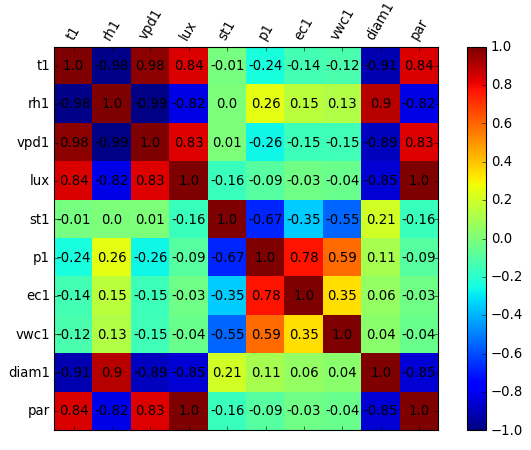
\includegraphics[width=10 cm]{4_ChapterMaterials/figuras/Correlation_matrix.png}
    \caption{Correlation Matrix from Paula Fernández Yepes thesis (2022)\cite{FernandezYepes2022}}
    \LABFIG{FIG}
    \end{figure}

The analysis revealed that the variables most closely correlated with plant diameter include air temperature (t1), relative humidity (rh1), vapor pressure deficit (vpd1), light intensity (lux), and photosynthetically active radiation (PAR). These findings highlight the significant role these variables play in influencing plant growth dynamics.

For instance, air temperature is a critical factor affecting photosynthesis, respiration, and transpiration, all of which are directly linked to the plant's growth rate and stem expansion. Similarly, relative humidity impacts the plant's water use efficiency and can lead to either water stress or fungal diseases depending on its level, thus influencing the plant's structural development. Additionally, light intensity, measured as lux, is directly associated with the rate of photosynthesis, making it a key driver of biomass accumulation and stem diameter increase. The study also indicated that PAR is highly similar to lux in its correlation with plant diameter, suggesting that including both might introduce redundancy into the model. Therefore, choosing between lux and PAR is necessary to avoid multicollinearity.

Furthermore, the analysis showed that soil temperature (st1) correlates strongly with soil permittivity (p1) and volumetric water content (vwc1), highlighting its role in root activity and nutrient absorption. However, given that our primary focus is the stem diameter, st1 is chosen for its unique impact on root-related growth factors. Additionally, electrical conductivity (ec1) serves as an indicator of soil salinity, which can affect nutrient uptake and osmotic balance, thereby influencing plant health and growth.

Based on these insights, the selected variables for our multivariable time series forecasting model are temperature (t1), relative humidity (rh1), light intensity (lux), soil temperature (st1), electrical conductivity (ec1), and stem diameter (diam1) as the target variable. This selection is supported by the correlation analysis and aligns with the physiological understanding that temperature, humidity, light, and soil conditions are critical determinants of plant growth. By focusing on these variables, the model aims to capture the essential environmental interactions that drive changes in plant stem diameter, providing a robust framework for predicting growth trends and optimizing agricultural practices.


\section{Software Implementation}

This section outlines the software environments used for developing and training our machine learning models. The choice of programming language and development tools is crucial for efficient machine learning experiments. We selected Python due to its versatility and extensive libraries. Anaconda and Spyder were used for model development, while Google Colab provided cloud-based resources and GPU acceleration for training. Below, we describe the features and configurations of these environments in our workflow.

\subsection{Anaconda and Spyder}

\subsubsection{Anaconda}

Anaconda is an open-source distribution of Python and R designed for scientific computing and data science. It simplifies package management and deployment, making it ideal for developing complex machine-learning models. Anaconda's package manager, Conda, handles library dependencies and versions, ensuring compatibility and preventing issues that often arise in machine learning projects. Anaconda allows users to create isolated environments for different projects, maintaining specific package versions separately to avoid conflicts. This capability makes development smoother and more efficient. Additionally, Anaconda includes popular data science libraries such as NumPy, pandas, Matplotlib, and Scikit-learn, streamlining the setup process and saving time. Its cross-platform compatibility across Windows, macOS, and Linux ensures projects can be developed and executed on different operating systems without compatibility issues. In our project, Anaconda served as the primary tool for managing dependencies, providing a reliable framework for model training and evaluation.

\subsubsection{Spyder}

Spyder is an open-source Integrated Development Environment (IDE) for Python, specifically designed for data analysis, and is part of the Anaconda distribution. It includes integrated tools for data analysis, such as a variable explorer for inspecting data frames and arrays, and an interactive console for testing code snippets. These tools make data manipulation easier, enhancing the overall development process. Spyder also offers advanced debugging capabilities, which are essential for identifying and resolving issues in complex algorithms. Although primarily a Python IDE, Spyder supports several programming languages, making it versatile for scientific computing. Its customizable interface allows users to tailor the environment to their preferences, optimizing workflow during development. Spyder was the primary IDE during the initial phases of model development for our project. Its intuitive interface and powerful debugging tools were invaluable in writing and testing the initial versions of our algorithms. The variable explorer was particularly useful in visualizing datasets and intermediate results, providing insights that guided our modeling decisions.


\subsection{Google Colab}

Google Colab is a free cloud-based Jupyter notebook environment that allows developers to write and execute Python code through a browser. It has gained significant popularity in the data science community due to its accessibility and ease of use, allowing users to leverage powerful computational resources without needing local hardware. For our project, Google Colab was crucial for model training and experimentation, providing an efficient and flexible environment. As a cloud-based platform, Google Colab enables code execution without local resources, making it highly accessible to anyone with an internet connection. This eliminates the need for expensive hardware, enabling complex computations from virtually any location. Colab comes with many pre-installed machine learning libraries, such as TensorFlow, PyTorch, and Keras, reducing the time spent on setup and allowing researchers to focus on developing and testing models. Additionally, Google Colab integrates seamlessly with Google Drive, simplifying data storage and retrieval. This integration streamlines the management of large datasets, allowing users to access and manipulate data directly from their Google Drive accounts.

Google Colab also offers free access to GPU and TPU resources, significantly enhancing computational capabilities for training complex models. This support allows developers to run demanding computations at no cost, making it an attractive option for those needing to train deep learning models or perform other resource-intensive tasks.


\subsubsection{T4 Hosted Runtime Environment}

For this project, the T4 GPU runtime environment was utilized within Google Colab to significantly enhance the performance of our machine-learning models. The T4 GPU, part of NVIDIA's Tesla product line, is optimized for machine learning tasks, offering accelerated performance in model training and inference. This powerful GPU reduces training time for complex models, which is particularly beneficial for deep learning experiments where computational demands are high, enabling quicker and more efficient results.

\begin{figure}[htbp]
    \centering
    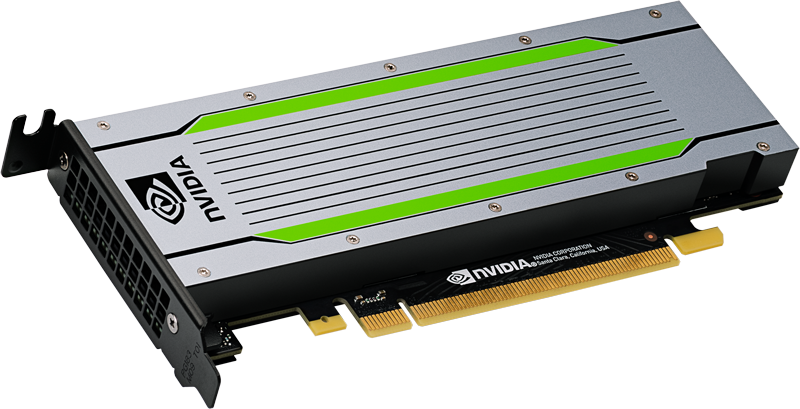
\includegraphics[width=6 cm]{4_ChapterMaterials/figuras/T4.png}
    \caption{NVIDIA T4 Tensor Core GPU}
    \LABFIG{FIG}
    \end{figure}

One of the significant advantages of using the T4 GPU is its cost efficiency. By leveraging Google Colab's free tier, we accessed this powerful hardware without additional costs, allowing extensive experimentation while staying within budget constraints. This economic aspect made the T4 GPU ideal for our project, providing high-level performance without the financial burden typically associated with advanced technology. The T4 GPU also offers excellent scalability, accommodating larger datasets and more complex neural networks. This scalability is crucial for modern machine-learning applications, where data volumes can be vast, and model architectures are increasingly intricate. The T4 GPU environment in Google Colab was instrumental during the training phases of our machine-learning models. Its powerful hardware accelerated the training process, enabling rapid iteration and optimization of our algorithms. The ability to quickly switch between different runtime environments and integrate with cloud storage facilitated a seamless workflow, allowing efficient experimentation and model refinement. This flexibility and ease of use were essential in achieving our project objectives, making the T4 GPU an invaluable resource throughout our development process.

\section{Python Libraries}

In the development of this project, several Python libraries were utilized to enhance functionality, streamline processes, and ensure efficient data handling. These libraries provided robust tools for various tasks, ranging from data manipulation and visualization to machine learning and statistical analysis. Next, I will explain the libraries used in this project.

\begin{enumerate}
    \item \textbf{gluonts} is a library for time series forecasting developed by Amazon. It excels in probabilistic forecasting, providing tools to create, evaluate, and deploy models with uncertainty estimates. This makes it ideal for applications like demand forecasting and financial analysis. GluonTS supports a range of forecasting models, from classical to deep learning, and integrates with MXNet for custom model building.
    
    \item \textbf{functools} is a Python Standard Library module for higher-order functions that work on or return other functions. It includes tools like \texttt{partial} for fixing function arguments, \texttt{lru\_cache} for caching results, and \texttt{reduce} for applying a rolling computation. It's useful for optimizing performance, writing modular code, and managing repetitive operations.
    
    \item \textbf{pandas} is a versatile library for data manipulation and analysis. It offers \texttt{DataFrames} and \texttt{Series} for efficient data handling, including features for data cleaning, transformation, and visualization. Pandas is essential in data science for managing and analyzing large datasets from various sources like CSV, Excel, and SQL databases.
    
    \item \textbf{matplotlib} is a library for creating static, interactive, and animated visualizations. It supports a range of plots, including line graphs, bar charts, and 3D plots. Matplotlib is crucial for data visualization in scientific computing and machine learning, allowing extensive customization of plots and integration with libraries like NumPy and Pandas.
    
    \item \textbf{scipy} extends NumPy with a broad range of functions for advanced mathematics, science, and engineering. It includes modules for optimization, integration, interpolation, and statistics. SciPy is widely used in fields like bioinformatics and physics for simulations, data analysis, and model fitting.
    
    \item \textbf{sklearn} (or \textbf{scikit-learn}) is a user-friendly library for machine learning. It provides tools for classification, regression, clustering, and dimensionality reduction, along with model selection and preprocessing utilities. Scikit-learn integrates well with NumPy, SciPy, and Matplotlib, making it a go-to for machine learning projects.
    
    \item \textbf{numpy} is fundamental for numerical computing in Python, supporting arrays and matrices with a wide array of mathematical functions. NumPy is crucial for handling large datasets and performing complex numerical operations efficiently, serving as the foundation for many scientific computing libraries.
    
    \item \textbf{typing} adds support for type annotations in Python, allowing developers to specify expected data types for variables and functions. This improves code clarity and reduces runtime errors, particularly in large or collaborative projects. Typing also facilitates the use of static type checkers like \texttt{mypy}.
    
    \item \textbf{torch} (or \textbf{PyTorch}) is a deep learning library developed by Facebook. It is known for its dynamic computation graph, which makes model building and experimentation flexible. PyTorch supports a wide range of neural network architectures and integrates with GPU acceleration for efficient training of large-scale models.
    
    \item \textbf{math} is a module providing basic mathematical functions and constants, such as trigonometric functions, logarithms, and square roots. It is useful for both simple calculations and more complex algorithms, making it a fundamental tool for anyone working with numerical data in Python.
    
    \item \textbf{Hugging Face Libraries:} Hugging Face offers a suite of open-source libraries designed to simplify the development and deployment of machine learning models. These libraries include:
    \begin{itemize}
        \item \textbf{datasets:} This library makes it easy to access and manipulate datasets for training machine learning models. It provides a standardized way to load, preprocess, and work with a variety of datasets, streamlining the data preparation process.
        \item \textbf{transformers:} This library provides implementations of transformer-based models for natural language processing (NLP), such as BERT, GPT-3, and others. It offers pre-trained models and tools to fine-tune them for various NLP tasks, enabling advanced text analysis and generation.
        \item \textbf{accelerate:} This library facilitates distributed training and the use of hardware accelerators like GPUs and TPUs. It simplifies the process of scaling up model training and utilizing high-performance hardware, improving efficiency and speed.
        \item \textbf{evaluate:} This library provides metrics and tools for assessing the performance of machine learning models. It helps in evaluating models against benchmarks and understanding their effectiveness in various tasks, aiding in model selection and improvement.
    \end{itemize}
\end{enumerate}
